\documentclass[11pt, a4paper]{report}

\usepackage{graphicx}
\graphicspath{ {images/} }
\usepackage{caption}
\usepackage{subcaption}

\usepackage{hyperref}
\usepackage[xindy]{glossaries}
\makeglossaries
\makeindex

\usepackage[utf8]{inputenc}
\usepackage{csquotes}

\usepackage[square,sort,comma,numbers]{natbib}
\bibliographystyle{IEEEtran}

\usepackage{amsmath}
\newcommand\addtag{\refstepcounter{equation}\tag{\theequation}}
\usepackage{txfonts}

\setlength{\parindent}{0ex}
\setlength{\parskip}{1ex}

%Rechtangle painting
\usepackage{tikz}
\usepackage[framemethod=tikz]{mdframed}

\mdfdefinestyle{mdthight}{
    linewidth=1pt,
    innerleftmargin=0bp,
    innerrightmargin=0bp,
    innertopmargin=0bp,
    innerbottommargin=0bp
}

\begin{document}
\begin{titlepage}
    \title{IP6 - Report Street Networks}
    \date{\today}
    \author{J. Peyer, S. Merki}
    \maketitle
\end{titlepage}
\setcounter{page}{1}

\tableofcontents


\begin{abstract}
    Text here.
\end{abstract}

\chapter{Introduction}
To analyse and generate streets there are many approaches. Street networks can be described as grammars. 

The street networks can be separate into reasonable parts by clustering algorithms. 

The cluster can be evaluate by measurement methods provided by the architecture department of the ETH-Zurich. 
(Insert here how our work is used later!)
Genetic analysis of street network, separation, recombination.
\chapter{Theoretical Task}
\section{Street Network Grammars}
\subsection{Shape Grammar}
The main key of shape grammar is to generate paintings by a new defined grammar based on shapes, selection rules, painting rules and limiting shapes. Shape grammar is a language based on an alphabet of shapes and generated shapes \citep{shapeGrammars:1972}. 

A class of paintings defines the pair (S,M). S represents the Shape specifications and M the material specifications. The Shape specification contains a shape grammar, defining a language of two dimensional shapes, and a selection rule. M specifies a finite list of material specifications and one limiting shape on a canvas.

\subsubsection{Shape Grammar Definition}
\label{sec:Shape_Grammar_Definition}
Shape Grammar is defined over an alphabet of shapes and generated n-dimensional shapes\citep{shapeGrammars:1972}.
\begin{displayquote} 
    Definition. A shape grammar (SG) is a 4-tuple: $SG = (V_T, V_M, R, I)$ where
    \begin{enumerate}
        \item $V_T$ is a finite set of shapes.
        \item $V_M$ is a finite set of shapes such that $V_T $* $\cap$  $V_M = \emptyset$
        \item R is a finite set of ordered pairs (u.v) such that u is a shape consisting of an element of $V_T $* combined with an element of $V_M$ and v is a shape consisting of (A) the element of $V_T $* contained in u or (B) the element of $V_T $* contained in u combined with an element of $V_M$ or (C) the element of $V_T $* contained in u with an additional element of $V_T$* and an element of $V_M$.
        \item I is a shape consisting of elements of $V_T $* and $V_M$.
    \end{enumerate}
\end{displayquote}

\subsubsection{Selection Rules}
\label{sec:Shape_Grammar_Selection_Rules}
An undefined count of shape rules provide the generation of the painting. Therefore a mechanism to select a correct shape is required. The depth is defined by levels witch is being assigned during generation based on there rules:\citep{shapeGrammars:1972}.
\begin{displayquote}
    \begin{enumerate}
        \item The terminals in the initial shape are assigned level 0.
        \item If a shape rule is applied, and the highest level assigned to any part ot the terminal corresponding to the level side of the rule is N, then
        \begin{enumerate}
            \item If the rule is of type A, any part of the terminal enclosed by the marker in the left side of the rule is assigned N.
            \item If the rule is of type B, any part of the terminal enclosed by the marker in the left side of the rule is assigned N and any part of the terminal enclosed by the marker is assigned N+1.
            \item If the rule is of type C, the terminal added is assigned N+1.
        \end{enumerate}
        \item No other level assignments are made.
    \end{enumerate}
\end{displayquote}

\subsubsection{Painting Rules}
\label{sec:Shape_Grammar_Painting_Rules}
Painting rules describe witch shape should be painted inside of a defined area. Like in a Venn diagram the rules contain multiple levels 0 - n. By combining this levels the painting colour is described\citep{shapeGrammars:1972}.
\begin{displayquote}
    A painting rule has two sides separated by a double arrow ($\Rightarrow$). The left side of a painting rule defines a set using the sets determined by level assignment and the usual set operators, for example, union($\bigcap$), intersection ($\bigcup$), complementation($\sim$), and exclusive or ($\bigotimes$), The sets defined by the left side of the painting rules of M must partition the universal set. The right side of a painting rule is a rectangle painted in the manner the set defined by the left side of the rule is to be painted.
\end{displayquote}

\subsubsection{Limiting Shapes}
\label{sec:Shape_Grammar_Limiting_Shapes}
These Shapes define a limiting area on the canvas, where shape painting is allowed. 
The area could have any form, but normally it is defined as a rectangle. Like a camera view the Limiting Shape define the scale of a painting and its viewpoint. Therefore the initial/start shape could be outside of the limiting shape 

\subsubsection{Example\citep{shapeGrammars:1972}}
\paragraph{Shape Grammar}
\begin{align}
\label{eq:Shape_Grammar}
SG1 &= <V_T, V_M, R, I>  \\
\label{eq:Shape_Grammar_VT}
V_T &= \{-\}  \\
\label{eq:Shape_Grammar_VM}
V_M &= \{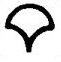
\includegraphics{sg_specification_VM.jpg} \}\ \\
\label{eq:Shape_Grammar_R}
R &= Rules\ [R]\ \ \ \ 
R1=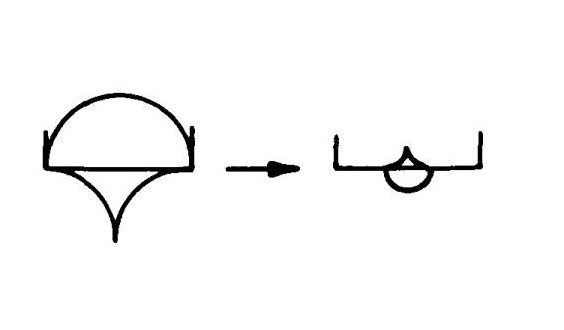
\includegraphics[width=2cm]{sg_specification_rule1.jpg}
R2=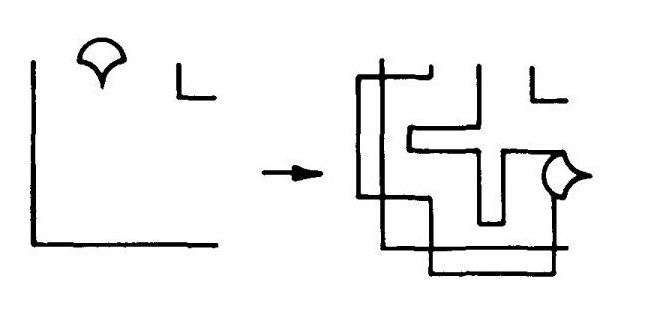
\includegraphics[width=2cm]{sg_specification_rule2.jpg}
R3=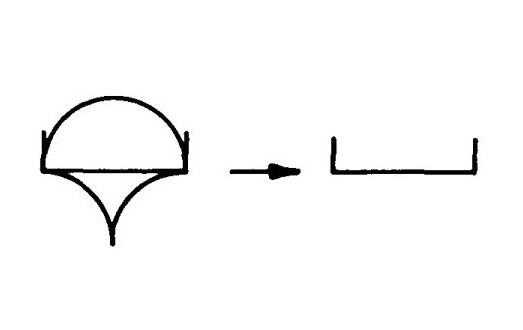
\includegraphics[width=2cm]{sg_specification_rule3.jpg}
\\
\label{eq:Shape_Grammar_I}
I &= Initial\ Shape\ I\ \ 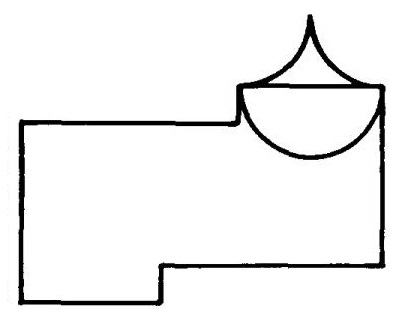
\includegraphics[width=1.5cm]{sg_specification_I.jpg}
\end{align}
\paragraph{Selection Rule}
\begin{equation}
<0,2>
\end{equation}

\paragraph{Painting Rules}
\begin{align}
    \label{fig:Shape Grammars/Shape Specification/Painting_Rule_1}
    L0\cap L1\cap L2 \Longrightarrow  
    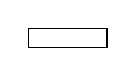
\begin{tikzpicture}
        \filldraw[fill=black!00!white, draw=black] (0,0) rectangle (1,0.25);
    \end{tikzpicture} \\
    \label{fig:Shape Grammars/Shape Specification/Painting_Rule_2}
    (L0\cap L1\cap \sim L2)\cup (L0\cap \sim L1\cap L2)\cup (\sim L0\cap L1 \cap L2) \Longrightarrow  
    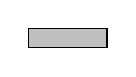
\begin{tikzpicture}
        \filldraw[fill=black!25!white, draw=black] (0,0) rectangle (1,0.25);
    \end{tikzpicture} \\
    \label{fig:Shape Grammars/Shape Specification/Painting_Rule_3}
    (L0\cap \sim L1\cap \sim L2)\cup (\sim L0\cap L1\cap \sim l2)\cup (\sim L0\cap \sim L1 \cap L2) \Longrightarrow  
    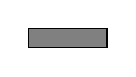
\begin{tikzpicture}
        \filldraw[fill=black!50!white, draw=black] (0,0) rectangle (1,0.25);
    \end{tikzpicture} \\
    \label{fig:Shape Grammars/Shape Specification/Painting_Rule_4}
    \sim (L0\cup L1\cup L2)  \Longrightarrow  
    
\begin{tikzpicture}
        \filldraw[fill=black!100!white, draw=black] (0,0) rectangle (1,0.25);
    \end{tikzpicture}
\end{align}
\paragraph{Limiting Shape}
\begin{figure}[!h]
    \centering
    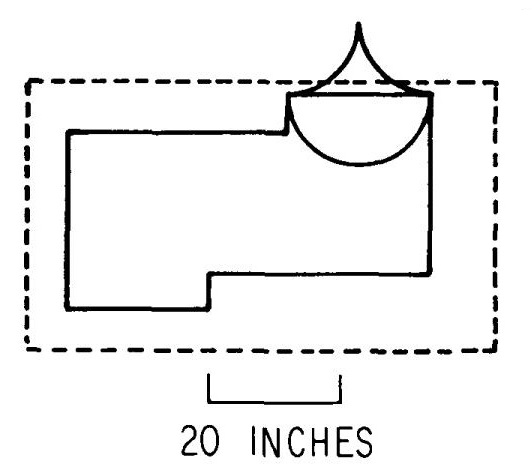
\includegraphics[width=2cm]{sg_specification_Limiting_shape.jpg}
    \caption{ Limiting Shape I \citep{shapeGrammars:1972}}\label{fig:Shape Grammars/Shape Specification/Limiting_Shape}
\end{figure}
\pagebreak
\paragraph{Generated}
The following image \ref{fig:Shape Grammars/Example} shows the generated painting with the relevant Steps. The levels are generated like described above \ref{sec:Shape_Grammar_Selection_Rules} 
\newline
Level 0: Steps 0 to 2,\newline Level 1: Steps 3 and 4,\newline Level 2: Steps 18 and 19
\begin{figure}[!h]
    \centering
    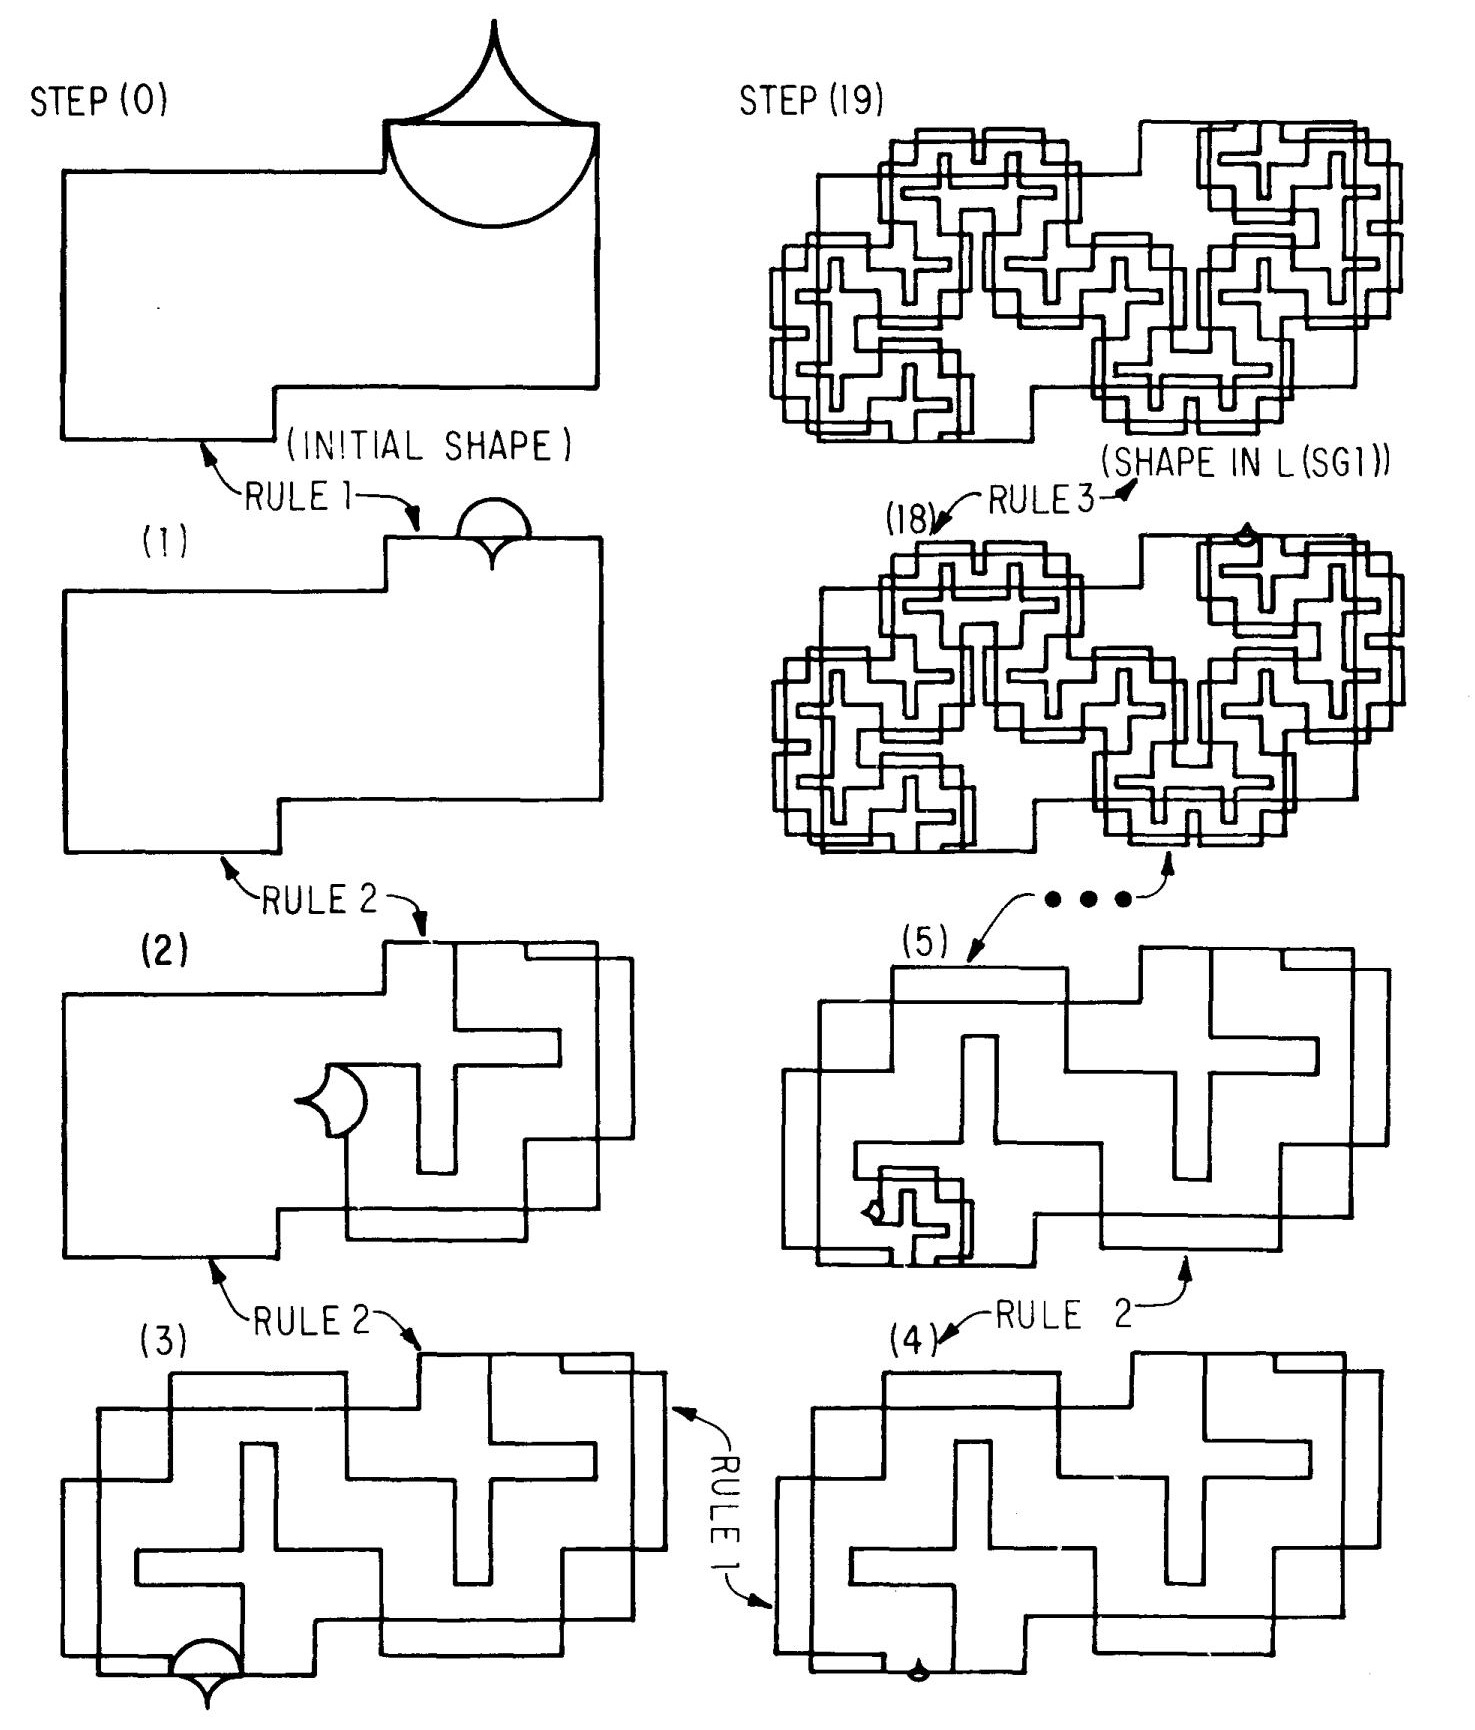
\includegraphics{sg_example.jpg}
    \caption{ Generated Painting\citep{shapeGrammars:1972}}\label{fig:Shape Grammars/Example}
\end{figure}

\pagebreak
\subsubsection{Street Generation}
In the following section we compare arguments for and against the usefulness to generate street networks by Shape Grammar. 
\paragraph{Features}
    \begin{itemize}
        \item Can describe and generate facedes in high details.
        \item With R Shapes windows and hight detail 3D Models can be generated easily.
    \end{itemize}

\paragraph{Problems}
    \begin{itemize}
        \item The generates streets result mostly in monotonous streets. 
        \item A huge number of R shapes is needed to generate a street network.
        \item Areas with different characteristics (historic district, rectangular raster like New York or radial to center like Paris) are difficult to generate.
        \item The R rules for the transitions between area characteristics are should not repeat themselves and are therefore difficult to build.
    \end{itemize}

\pagebreak
\subsection{L-Systems}
L-System is a well established modelling approach for the synthesis of realistic plant images. There are many papers describing L-Systems and how they are applied to generate plant live: "In these cases L-System productions capture the \textit{development} of plant components over time." \citep{PrusinkiewiczEtAl:2001} Productions are applied in parallel, so that all plant parts grow and age equally. The growth is stopped at a defined terminal age. This age is the number of iterations, where in each iteration productions are applied.

The context-free productions in \citep{PrusinkiewiczEtAl:2001} are defined using the following syntax.
\begin{equation} \label{eq:lsystem context free}
    pred : \{block1\}\ cond\ \{block2\} \leadsto succ
\end{equation}
The symbol \textit{pred} (predecessor) defines the module that will get replaced by the modules defined in \textit{succ} (successor). This replacement is only applied, if the (optional) condition is met. \textit{block1} and \textit{block2} are C statement blocks, of which the first block is executed before and the second after the condition is evaluated. \citep{PrusinkiewiczEtAl:2001} gives the following example.
\begin{equation} \label{eq:lsystem example 1}
    A(x) : \{y = x + 2;\}\ y \geq 5\ \{z = y / 3;\}\ \leadsto B(z)C(z + 1)
\end{equation}
If this example production was applied to the module $A(4)$, it would result in the modules $B(2)C(3)$.

The cpfg language, described in \citep{PrusinkiewiczEtAl:2001}, also supports context-sensitive productions. The following listing defines the syntax of such a production.
\begin{equation} \label{eq:lsystem context sensitive}
    lcont < pred > rcont : \{block1\}\ cond\ \{block2\} \leadsto succ
\end{equation}
\textit{lcont} (left context) and \textit{rcont} (right context) each define a list of modules that have to precede or respectively follow the \textit{pred} (module being replaced). Context modules are limited to query symbols, which are explained later on. \citep{PrusinkiewiczEtAl:2001} gives the following example.
\begin{equation} \label{eq:lsystem example 2}
    A(x) < B(y) > C(z) : x + z > 0 \leadsto M(y / 2)N(y / 2)
\end{equation}
If the example of listing \ref{eq:lsystem example 2} was applied to the module composition $A(2)B(4)C(0)$, it would result in the modules $A(2)M(2)N(2)C(0)$.

A way to generate images with L-Systems is to use a LOGO-style turtle as a graphical model. Certain modules of the L-System are interpreted as commands to this turtle.

\pagebreak
\subsection{Space Syntax}
The grammar Space Syntax was first introduced 1976 by B. Hiller, A. Leaman, P. Stansall and M. Bedford in the paper "Space syntax" \citep{spaceSyntax:1976}. The grammar is a morphic language and describes methods to analyse and generate urban areas and buildings.
The language consists of a surface space and an ongoing production process of new and different neighbouring parts. Extended Syntax is used to describe special area pattern like ring spaces and block spaces.

The grammar was later extended and integrated into Geographic Information System (GIS). This information systems are used to plan and analyse the human interaction with the environment. 
Bin Jiang and Christope Claramunt \citep{integrationSpaceSyntaxGIS:2002} showed the limitation of axial lined-based space syntax (\citep{integrationSpaceSyntaxGIS:2002} chapter: 2.2). They then created a graph representation (\citep{integrationSpaceSyntaxGIS:2002} chapter: 3) and showed that it was at least equivalent to the predefined syntax created by B. Hiller et al.\citep{spaceSyntax:1976}.

Many projects has bean developed based on the space syntax graph representation. 

\pagebreak
\section{Clustering Algorithms}
In the application CPlan as described in \ref{CPlan} the street network is generated as a graph. To separate and select areas with specific characteristics we tried machine learning clustering algorithms. In this section the different clustering algorithms are analysed and the generated results produced by our implementations in CPlan are compared.
\subsection{K-Means}
\subsubsection{Description}
The K-Means algorithm detects the clusters / partitions by measuring the euclidean distance between the cluster centroids and the position of the street junctions. The algorithm uses the following approach:

\begin{enumerate}
    \item A number of points are inserted into the graph and used as centroids.
    \item All graph points are assigned to their nearest centroids.
    \item The centroids are moved to the center of their assigned graph points.
    \item Until the maximum number of iterations is reached: Continue the loop with item 2.
\end{enumerate}
Because the K-Means algorithm can find local minima, this process needs to be executed more than once. The result with the best found solution will be selected.

\subsubsection{Implementation}
We implemented in CPlan\citep{cPlan:2015} an optimised version of the described algorithm based on the paper An Efficient k-Means Clustering Algorithm: Analysis and Implementation \cite{kmeans:2002} with a runtime of $O(n\ insert\ here)$

\subsubsection{Speed Optimization}
The ETH-Zurich provided the following networks: Bad Berka (552 nodes, 626 edges), Weimar (2012 nodes, 2646 edges) and Zurich (27446 nodes, 35121 edges). The network Zurich with factor 13 more edges than Weimar resulted in long processing time. A speed improvement can be achieved by running the K-Means iterations in parallel. Every iteration can be executed side effects free. The measurements and comparisons of the results are provided in the section Practical Task/Measurements \ref{sec:measurements};

\pagebreak
\subsubsection{Result}
Our implementation in CPlan\ref{CPlan} has produced the following image\ref{fig:KmeansGenerated}. All streets in one cluster are marked with the same colour, the transitions between clusters are marked black.
\begin{figure}[!h]
    \centering
    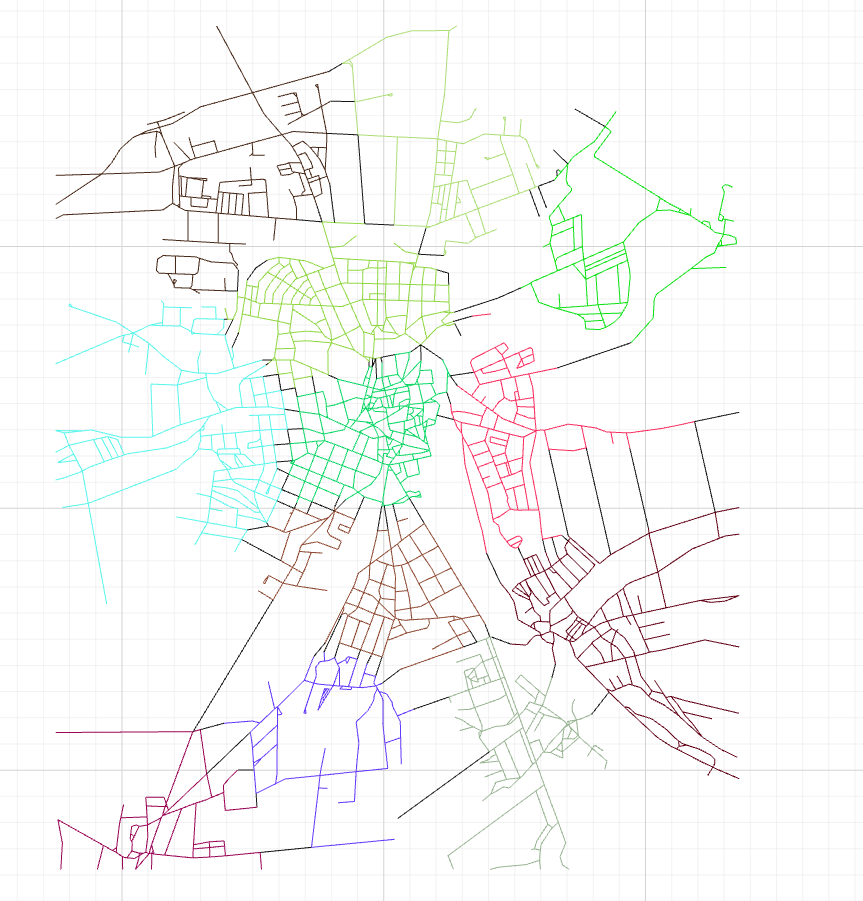
\includegraphics[width=\textwidth]{clusteranalysis_kmeans_result.png}
    \caption{K-Means cluster analysis of Weimar\label{fig:KmeansGenerated}}
\end{figure}
\pagebreak
\subsubsection{Problems}
Because the algorithm uses the euclidean distance between cluster centroids and street junctions, the edge data (e.g. street length) is not used. This leads therefore to unexpected transitions between clusters.
\begin{figure}[!h]
    \centering
    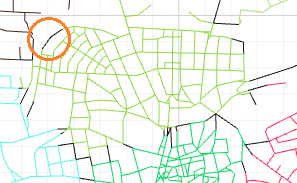
\includegraphics[width=0.5\textwidth]{clusteranalysis_kmeans_problem.png}
    \caption{Problem of K-Means clustering\label{fig:KmeansProblem}}
\end{figure}
\newline
If a point has only connections into another cluster, the result are many unexpected transitions. The result can be seen in the figure\ref{fig:KmeansProblem} in the read circle.
\pagebreak
\subsubsection{K-Means with Shortest Path}
To solve the problem of unexpected transitions between clusters the best result of the K-Means algorithm can be combined with the distance measurement of a shortest path algorithm (in our example Dijkstra or FloydWarshall). The edges are assigned by the edge data (e.g. street length) to the nearest cluster. Therefore the result is a connected graph. This means every vertex can be reached from every other vertex within the a cluster.
\newline
Additional calculation time is needed for the shortest path algorithm. The differences can be compared in the section Practical Task/Measurements \ref{sec:measurements};

\begin{figure}[!h]
    \centering
    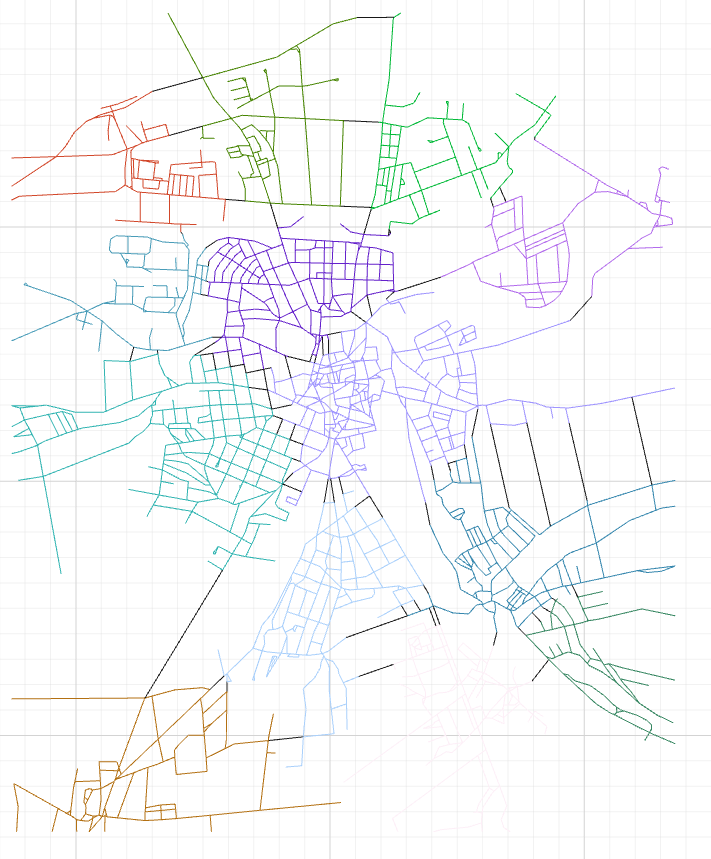
\includegraphics[width=0.9\textwidth]{clusteranalysis_kmeansExt_result.png}
    \caption{K-Means clustering with shortest path\label{fig:Kmeansshortestp}}
\end{figure}



\pagebreak
\subsection{Hierarchical Clustering}
\subsubsection{Introduction}
Hierarchical clustering, also known as connectivity based clustering, was the next used approach. This area of algorithms clusters nodes together, which are near to each other. The advantage over K-Means is that graph distances can be used instead of the euclidean distance.

The result of a hierarchical clustering algorithm is a tree (or hierarchy), hence the name. This result can be used to create 1 to n clusters, where n is the number of input nodes.

\subsubsection{Strategy}
There are generally two main strategies for hierarchical clustering:

\begin{itemize}
    \item \textbf{Agglomerative}: Bottom up strategy. In the beginning each node is an own cluster. Clusters are combined until only a single cluster remains.
    \item \textbf{Divisive}: Top down strategy. All nodes are contained in one cluster at the start. This cluster is then divided into sub clusters.
\end{itemize}

The time complexity of the divisive strategy is with $O(2^n)$ too bad for the size of the street networks on which the algorithms have to run. The agglomerative strategy runs in $O(n^2 log(n))$ and in some special cases in $O(n^2)$ time complexity. The hierarchical clustering algorithms implemented for this thesis run in $O(n^2)$ time complexity. They are based on the paper "Optimal implementations of UPGMA and other common clustering algorithms" \cite{clustering:2007}.

\subsubsection{Reduction Formula}
The reduction formula is used to determine the distance between two clusters.
The following reduction formulae were implemented for this thesis:

\begin{itemize}
    \item \textbf{Single Linkage}
    \begin{multline}
    D_{Single-Linkage}(C_1, (C_2 \cup C_3)) \leftarrow \\
    min \{ D_{Single-Linkage}(C_1, C_2), D_{Single-Linkage}(C_1, C_3) \}
    \end{multline}
    \item \textbf{UPGMA}
    \begin{equation}
    \begin{split}
    D_{UPGMA}(C_1, (C_2 \cup C_3)) \leftarrow &\frac{|C_2|}{|C_2|+|C_3|}D_{UPGMA}(C_1, C_2)\ + \\ &\frac{|C_3|}{|C_2|+|C_3|}D_{UPGMA}(C_1, C_3)
    \end{split}
    \end{equation}
    \item \textbf{WPGMA}
    \begin{equation}
    D_{WPGMA}(C_1, (C_2 \cup C_3)) \leftarrow \frac{1}{2} (D_{WPGMA}(C_1, C_2) + D_{WPGMA}(C_1, C_3))
    \end{equation}
\end{itemize}

With clusters $C_1$, $C_2$ and $C_3$, which are sets of nodes and the distance function $d(i, j)$, which determines the distance between nodes $i$ and $j$.

For every of these reduction formulae the following holds:

\begin{equation}
\begin{split}
&\textrm{let }C_1, C_2\textrm{ be clusters },i \in C_1, j \in C_2 \\
&\textrm{if }|C_1| = |C_2| = 1 \\
&\textrm{then }D(C_1, C_2) = d(i, j)
\end{split}
\end{equation}

For both the single linkage and the UPGMA reduction formula exists a dissimilarity function (\ref{eq:df_single_linkage} and \ref{eq:df_upgma}). These are alternative formulations of the reduction formulae which determine the distance by traversing all nodes of both clusters. The created cluster hierarchy is not used in these functions. For the WPGMA reduction formula no dissimilarity function exists, as shown in \cite{clustering:2007}.

\begin{equation} \label{eq:df_single_linkage}
D_{Single-Linkage}(C_1, C_2) = \min_{i\in{C1}, j\in{C2}}\{d(i, j)\}
\end{equation}
\begin{equation} \label{eq:df_upgma}
D_{UPGMA}(C_1, C_2) = \dfrac{1}{|C_1||C_2|} \sum_{i\in{C1}, j\in{C2}}{d(i, j)}
\end{equation}


\subsubsection{Single-Linkage Result}
The figure \ref{fig:SingleLinkage} shows the result of a hierarchical cluster analysis using the single linkage reduction formula. The used distance function $d(i, j)$ was the shortest distance from $i$ to $j$ in the street graph. As it is clearly visible when looking at the result, this way of cluster analysis is not creating the desired output. There is one huge cluster in the middle and many one-node clusters at the border of the city.

The problem is caused by the used reduction formula. Single linkage uses the distance between the closest nodes of the compared clusters. This leads to the creation of clusters, where all connecting roads are long. In a city, where there are multiple connections from one junction to another most of the time, this tends to create one-node clusters for nodes, which are connected to the city by a single long road.

\begin{figure}[!h]
    \centering
    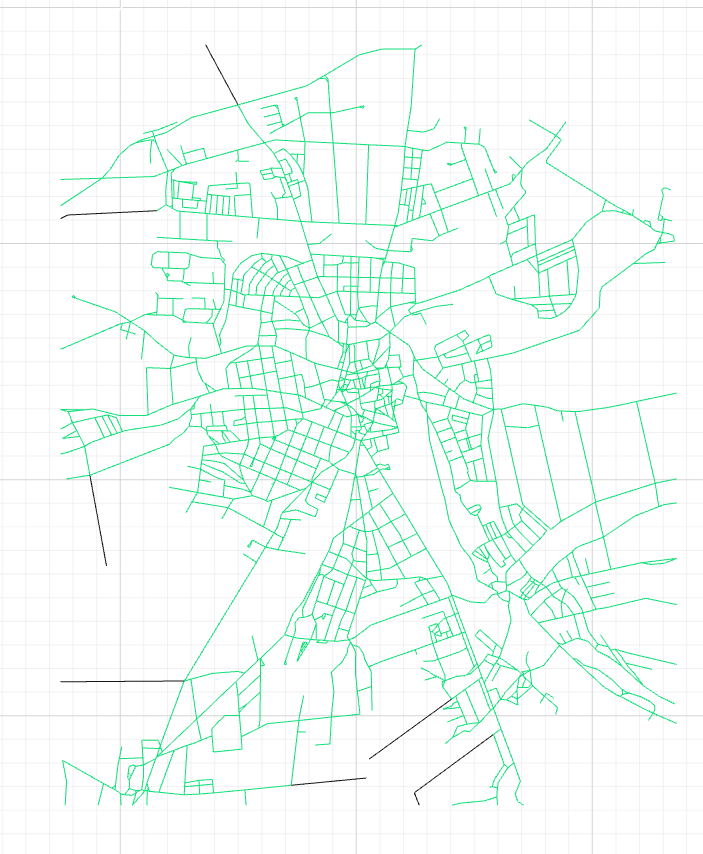
\includegraphics[width=\textwidth]{clusteranalysis_singlelinkage.png}
    \caption{Single-Linkage hierarchical cluster analysis of Weimar\label{fig:SingleLinkage}}
\end{figure}

\subsubsection{UPGMA and WPGMA Result}
%TODO: Add figure
The figures xxx and xxx show the result of hierarchical cluster analysis using the UPGMA, or respectively the WPGMA reduction formula. The same distance function $d(i, j)$ as in the single linkage solution was used (shortest distance from $i$ to $j$ in the street graph).

\pagebreak
\chapter{Practical Task}
\section{CPlan}\label{CPlan}
CPlan is a tool written by the Department of Architecture of the ETH-Zurich. The goal of this application is to generate/grow street networks dynamically and extend these networks with buildings. 
\subsection{Improvements}
\begin{itemize}
    \item Some calls to the methods IEnumerable.ToArray() and IEnumerable.ToList() were removed. This methods creates a new array / list and stores every item of the IEnumerable in this new collection. Therefore the application had an extremely large footprint. To further reduce this overhead some methods were changed to take IEnumerable parameters instead of arrays.
    \item Certain graph and geometry extension methods were fixed. It would be good practice to create unit tests for such methods.
    \item matrix2D not clockwise?
    \item Geometry2D not correct line intersection!
\end{itemize}

\subsection{Genetic algorithms}
The ETH-Zurich had already genetic optimizations algorithms based on trees. Unfortunately they had not a working solution to produce a tree from the existing graph. The new created tree generation produces a relative tree with absolute angles.

\subsection{Normalising Street Networks}
While testing clustering algorithms on the street network of Zurich one rough spot of this network was found: Not all streets, which lead to a junction are connected to it. As shown in figure \ref{fig:zuerich_error} there exist floating streets (highlighted in lime green). Both ends of these highlighted streets are not connected to the rest of the street network.

To handle those floating streets a network normalisation method was developed. The normalisation snaps (unites) all junctions and street end points, which are positioned close together, into one common junction. The result of this normalisation is shown in figure \ref{fig:zuerich_fixed}.

\begin{figure}[!h]
\begin{mdframed}[style=mdthight]
    \centering
    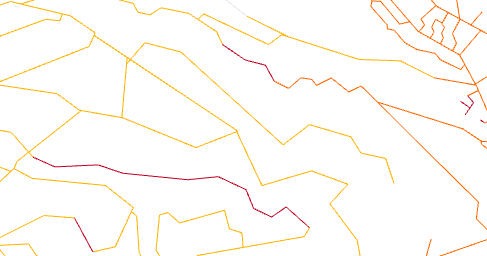
\includegraphics[width=\textwidth]{zuerich_street_error_cropped.png}
\end{mdframed}
    \caption{Floating streets in the street network of Zurich\label{fig:zuerich_error}}
\end{figure}

\begin{figure}[!h]
\begin{mdframed}[style=mdthight]
    \centering
    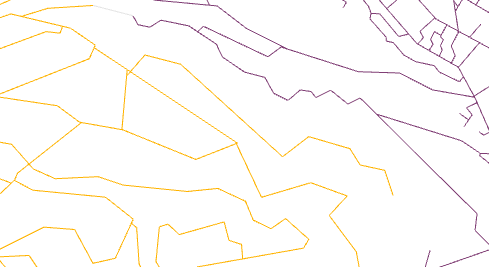
\includegraphics[width=\textwidth]{zuerich_street_fixed_cropped.png}
\end{mdframed}
    \caption{Normalised street network of Zurich\label{fig:zuerich_fixed}}
\end{figure}
\subsection{Cluster Detection}

\subsubsection{Measurements}
\label{sec:measurements}

\chapter{Conclusion}

\bibliography{quotations}
\appendix
\glsaddall
\printglossaries
\end{document}